Il programma sviluppato è stato progettato con l'obiettivo di fornire un framework di esecuzione per algoritmi che risolvono il \ddbpp. L'intento è creare un ambiente in cui, lo sviluppatore che voglia verificare le performance di un nuovo algoritmo, possa concentrarsi solo sullo sviluppo dello stesso, senza preoccuparsi di tutte le problematiche relative alla grafica o alla \emph{user experience}.

\subsection{Aspetto}
Ad un utente finale l'interfaccia grafica si presenta come in figura \ref{fig:main_window_ss}. Da questa finestra è possibile configurare le specifiche del problema quale dimensione dei contenitori, o \emph{bin}, e il numero di pacchetti, o \emph{packet}, con relative larghezze e altezze. Una volta configurato il problema, si potrà scegliere l'algoritmo, o \emph{Core}, con il quale risolverlo: ogni metodo risolutivo ha parametri di configurazione propri, mostrati nella sezione loro dedicata, che possono venir usati per adattare il comportamento dell'algoritmo alla specifica istanza. Una volta completata la fase di configurazione il \emph{Core} può essere lanciato e, ad ogni ottimo trovato, ne verrà visualizzato il \emph{placing}, il valore di fitness, il numero di iterazioni e il tempo impiegato per raggiungerlo.

\begin{figure}[h!tp]
 \centering
 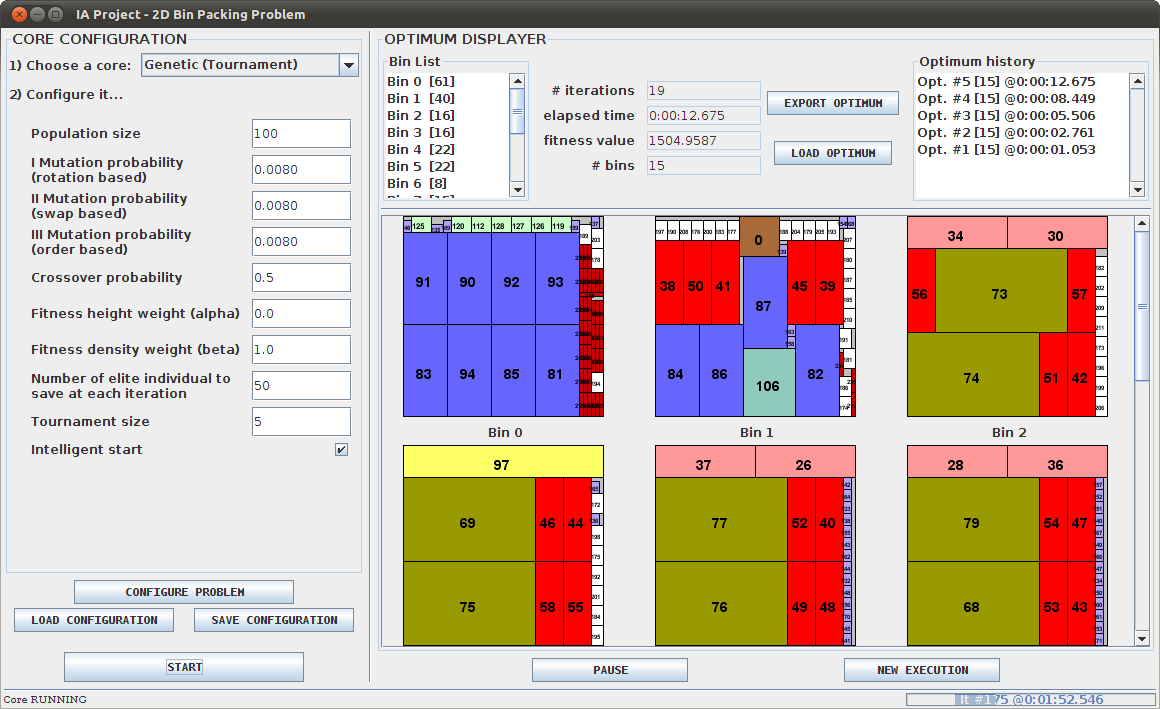
\includegraphics[width=\textwidth]{./img/main_window_ss.png}
 % main_window_ss.png: 1160x709 pixel, 72dpi, 40.92x25.01 cm, bb=0 0 1160 709
 \caption{Screenshot della finestra principale del programma}
 \label{fig:main_window_ss}
\end{figure}

\subsection{Caratteristiche peculiari}
Il framework sviluppato mette a disposizione diverse caratteristiche per facilitare l'utente finale nell'uso del software, così come lo sviluppatore nel test degli algoritmi.
\paragraph{Salvataggio \& caricamento della configurazione corrente}
Attraverso i pulsanti \texttt{SAVE} e \texttt{LOAD CONFIGURATION} è possibile salvare o caricare da file la configurazione del problema attualmente in esame, comprensiva del core selezionato e dei suoi parametri specifici. Il file prodotto sarà formattato secondo lo standard XML e modificabile anche al di fuori del programma.
\paragraph{Cronologia degli ottimi}
Ogni volta che l'algoritmo individua un nuovo ottimo la sua rappresentazione prende il posto della precedente. Questo comportamento può non essere sempre gradito in quanto uno sviluppatore potrebbe voler vedere l'intera evoluzione degli ottimi, per capire se l'algoritmo scritto si comporta nel modo correto, mentre un utente potrebbe accorgersi che, per una non precisa calibrazione della funzione di fitness, un ottimo precedente risulta ``più adatto agli scopi'' di quello successivo. Per porre rimedio a questo ostacolo il framework salva l'intera cronologia degli ottimi che possono così essere visualizzati nuovamente.
\paragraph{Salvataggio \& caricamento di ottimi}
I pulsanti \texttt{EXPORT} e \texttt{LOAD OPTIMUM} permettono all'utente di salvare qualsiasi ottimo presente nella cronologia, nonchè visualizzarlo nuovamente in futuro. Il file prodotto contiene la sequenza di bin con il \emph{placing} dei relativi pacchetti e, essendo in formato XML, può essere facilmente interpretato da un programma di terze parti.
\paragraph{Ingrandimento automatico dei \emph{bin}}
Da un punto di vista esclusivamente di \emph{user experience} la rappresentazione grafica dei \emph{bin} viene riscalata ogni volta che le dimensioni della finestra, e dei \emph{bin} stessi, lo permettono. Ciò facilita l'analisi dell'ottimo trovato soprattutto quando questo è composto da oggetti di piccole dimensioni.

\subsection{Classi essenziali}
L'aggiunta di nuovi \emph{Core} da parte di uno sviluppatore comincia con la comprensione dello schema UML presentato in figura \ref{fig:uml_classi}.
\begin{description}
	\item[\texttt{MainWindow}] gestisce la videata iniziale del programma, nonchè smista i flussi di informazioni provenienti dagli algoritmi in esecuzione e le interazioni con l'utente. Si incarica inoltre di gestire la configurazione dell'istanza del problema, fornendo questi dati ai \emph{Core} al momento opportuno.
	\item[\texttt{ProblemConfiguration}] definisce l'istanza specifica del problema: la gestione di questa classe è tutta a carico del framework e gli sviluppatori non dovranno far altro che usarla per attingere ai dati di cui hanno bisogno.
	\item[\texttt{GUISignaler}] fornisce ai \emph{Core} un modo per segnalare informazioni e anomalie nell'esecuzione.
	\item[\texttt{OptimumPainter}] è l'interfaccia che definisce qual'è il formato in cui i risultati dei \emph{Core} devono venir costruiti per essere visualizzati a video. Ciò non deve essere visto come una limitazione in quanto il framework prevede che gli sviluppatori possano usare i propri tipi di dato, avendo cura di creare una sorta di ``traduttore'' che converta i tipi specifici in quelli attesi dal metodo \texttt{paint} dell'interfaccia.
	\item[\texttt{CoreController}] mette a disposizione della \texttt{MainWindow} - e quindi dell'utente finale - gli strumenti per controllare e interagire con l'esecuzione dell'algoritmo.
	\item[\texttt{CoreDescriptor}] definisce le funzioni necessarie alla \texttt{MainWindow} per gestire i parametri di configurazione specifici di ogni \emph{Core} piuttosto che istanziarli fornendo loro le informazioni di cui hanno bisogno.
	\item[\texttt{AbstractConfigurator \& AbstractCore}] sono le due classi astratte che uno sviluppatore deve estendere per poter annettere il proprio core al framework. A seconda delle richieste della \texttt{MainWindow} \texttt{AbstractConfigurator} crea e restituisce il componente visuale contenente i parametri di configurazione del \emph{Core}, oppure istanzia la classe che implementa l'algoritmo vero e proprio, ritornandone il \texttt{CoreController} associato. \texttt{AbstractCore}, invece, è la classe da estendere per implementare l'algoritmo stesso. I vincoli a cui richiede di sottostare sono che l'algoritmo abbia una struttura ciclica, in cui ogni ciclo non richieda un eccessivo tempo di elaborazione, e che si fornisca il traduttore dai tipi di dato che rappresentano l'ottimo all'interno del \emph{Core} a quelli richiesti da \texttt{OptimumPainter}.
\end{description}


\begin{figure}[h!tp]
 \centering
 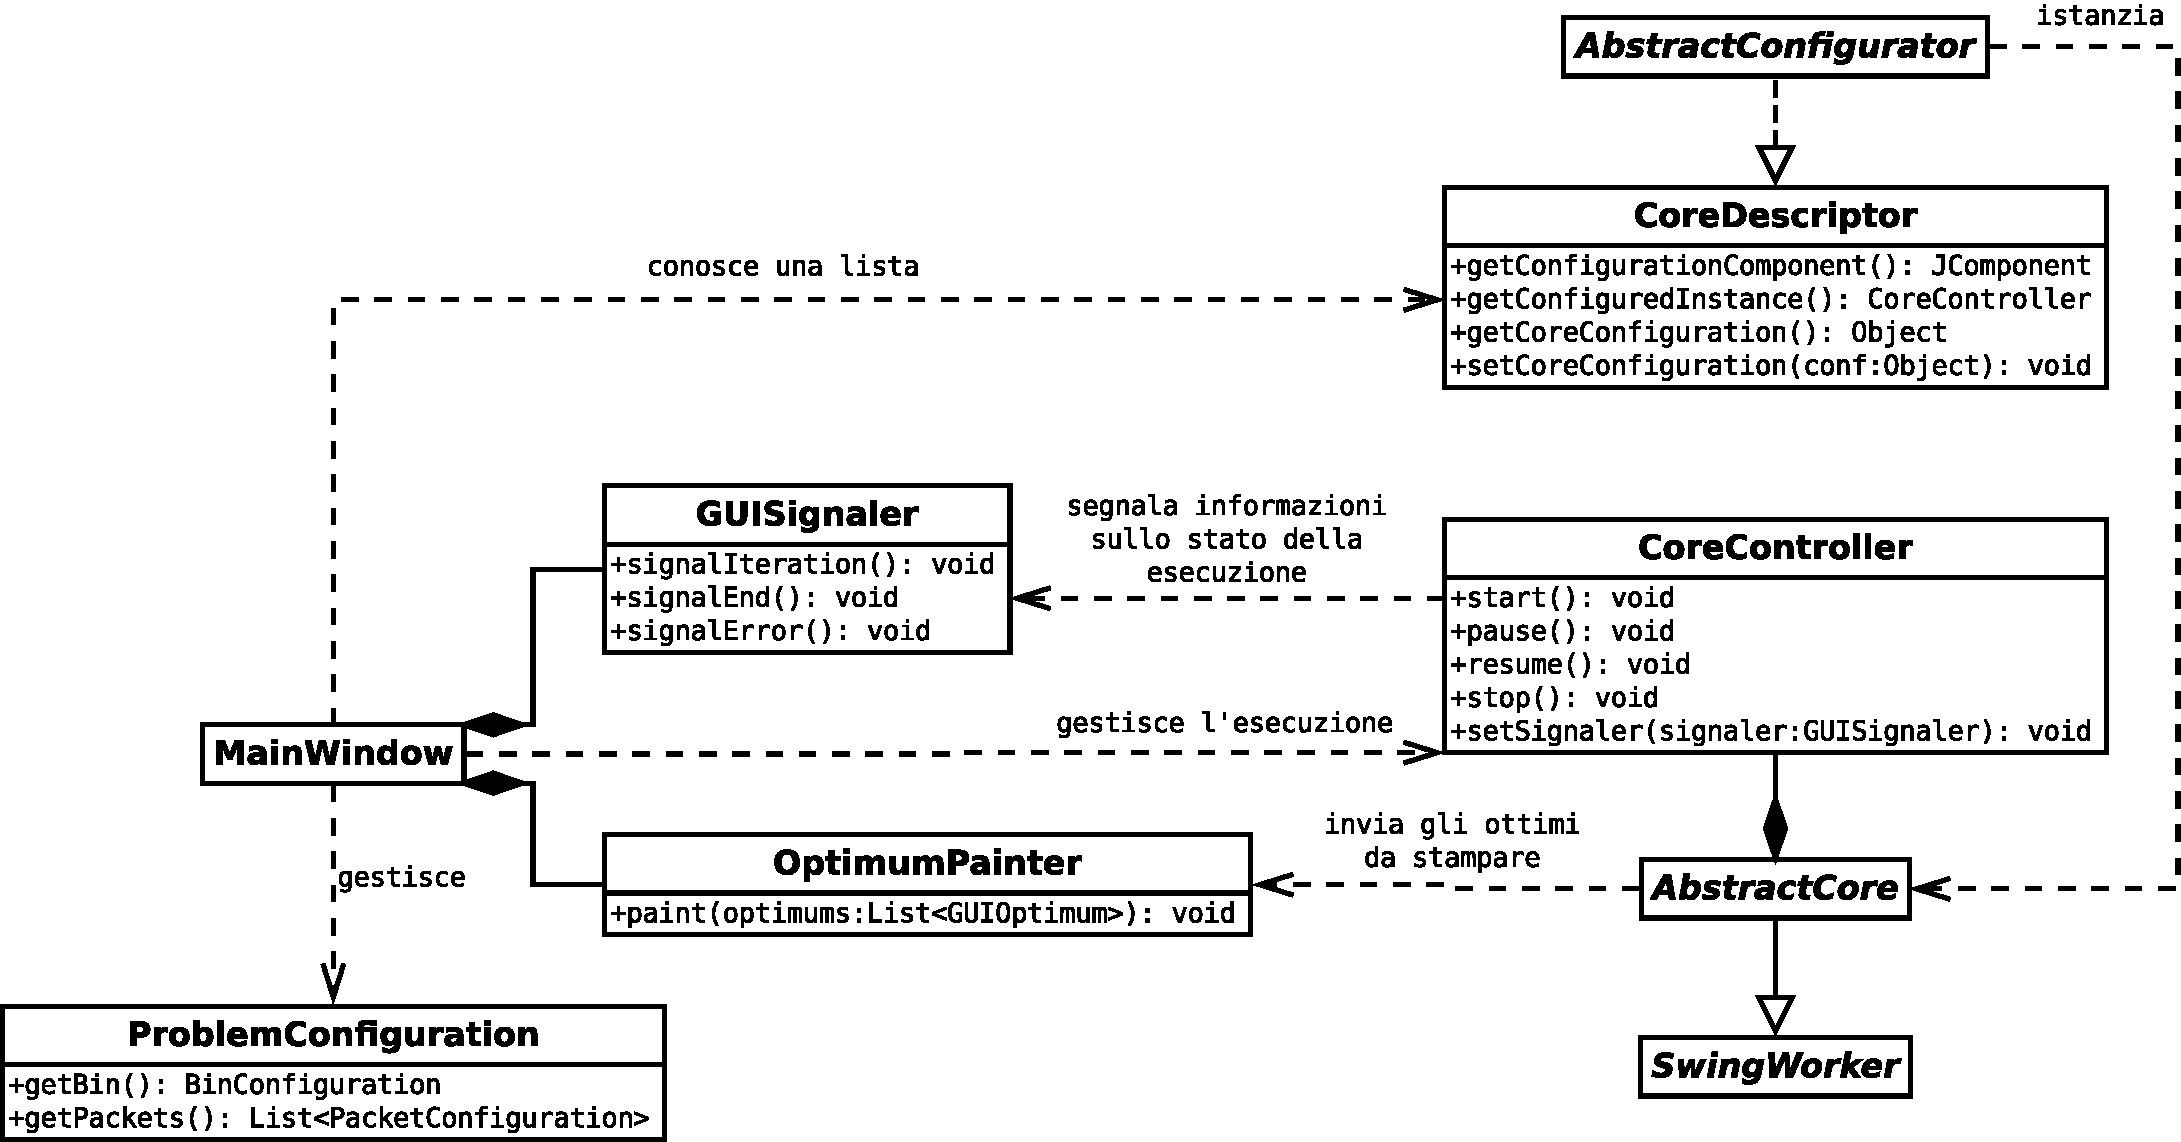
\includegraphics[width=\textwidth]{./img/uml_classi.pdf}
 % uml_classi.pdf: 1047x548 pixel, 72dpi, 36.94x19.33 cm, bb=0 0 1047 548
 \caption{Grafico UML delle classi principali dell'applicazione}
 \label{fig:uml_classi}
\end{figure}
